\subsection{Generación de señalamiento paso a paso}

	Al ejecutar el RNA, primero detectará todos los \textit{netElements}, sus coordenadas iniciales y finales en la topología, y el sentido en el que fueron definidas. El resultado obtenido se muestra en el Cóodigo \ref{lst:EJ2_1}.
	
	\begin{lstlisting}[language = {}, caption = Detección de \textit{netElements} por parte del RNA , label = {lst:EJ2_1}]
	###### Starting Railway Network Analyzer #####
	Reading .railML file
	Creating railML object
	Analysing railML object
	Analysing graph
	ne14 [-1521, 450] [-560, 450] >>
	ne15 [-1521, 300] [-560, 450] >>
	ne16 [-560, 450] [516, 450] >>
	ne17 [516, 450] [666, 300] >>
	ne18 [516, 450] [1521, 450] >>
	ne19 [666, 300] [28, 300] <<
	ne20 [666, 300] [1521, 300] >>
	The network is connected
	\end{lstlisting}

	Por ejemplo, el \textit{netElement} ne19 inicia en la coordenada (666;300) y finaliza en la coordenada (28;300). El símbolo $<<$ indica que ne19 se encuentra definido de derecha a izquierda , ya que la componente x de la coordenada final es menor a la de la coordenada inicial, teniendo la misma componente y. Además, se puede comprobar que la lista obtenida en consistente con la Figura \ref{fig:EJ2_2}. Por ejemplo, ne14, ne15 y ne16 comparten la coordenada (-560,450), que coincide con la coordenada del cambio de vías Sw01.
	
	A continuación, el RNA detectará la infraestructura ferroviaria, las curvas peligrosas y los puntos medios de los netElements que el RNA considera demasiado largos. El resultado de este proceso se puede visualizar en el Código \ref{lst:EJ2_2} y puede leerse también en el archivo Infrastructure.RNA.
	
	\begin{lstlisting}[language = {}, caption = Detección de puntos críticos por parte del RNA , label = {lst:EJ2_2}]
	Analysing infrastructure --> Infrastructure.RNA
	Detecting Danger --> Safe_points.RNA
	ne14 has a Platform[plf116] @ [-1075, -450]
	ne15 has a Curve(2 lines) @ [[-710, 300]]
	ne16 has a LevelCrossing[lcr120] @ [-192, -450]
	ne18 has a Platform[plf117] @ [1111, -450]
	ne19 has a Middle point @ [347.0, 300]
	ne20 has a Middle point @ [1093.5, 300]
	\end{lstlisting}

	Una vez que el RNA detectó cada punto crítico de la red ferroviaria, procede a generar el señalamiento. El orden de generación no es importante, pero para poder describirlo de forma consistente se iniciará generando el señalamiento para proteger los finales de vías, las junturas entre rieles, las plataformas, los cruces de vía y los cambios de vías. Luego se procederá a mostrar el señalamiento pre y post simplificación. Las señales generadas para proteger los finales de vías relativos y absolutos son ilustradas en la Figura \ref{fig:EJ1_3}.

	\begin{figure}[H]
		\centering
		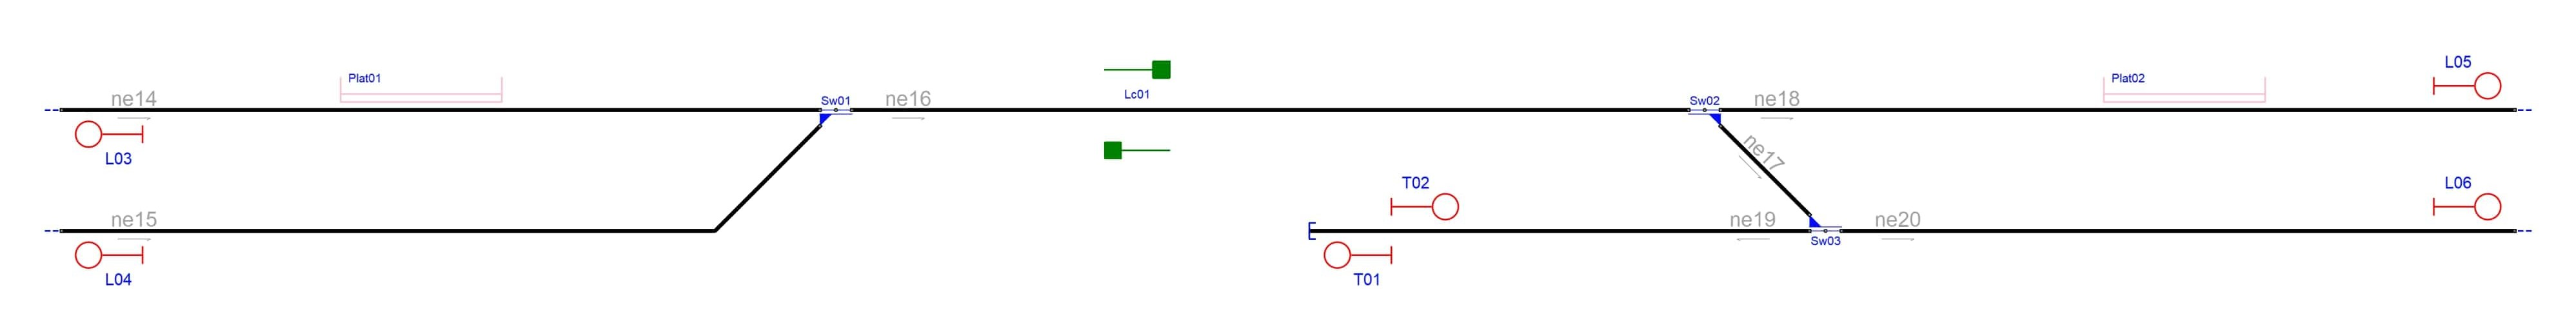
\includegraphics[width=1\textwidth]{resultados-obtenidos/ejemplo2/images/2_step1.png}
		\centering\caption{Señalamiento generado por el RNA para proteger el fín de vía.}
		\label{fig:EJ2_3}
	\end{figure}

	Los finales de vías absolutos son protegidos por la señal de parada T01 y la señal de partida T02. A su vez, los finales de vías relativos poseen las señales de parada L03, L04, L05 y L06, cercanos al límite del externo del \textit{netElement} al que pertenecen.

	La Figura \ref{fig:EJ2_3} ilustra la generación de señales destinadas a proteger las junturas entre los rieles. Al no existir junturas que proteger, el RNA salteará este paso.
	
	\begin{figure}[H]
		\centering
		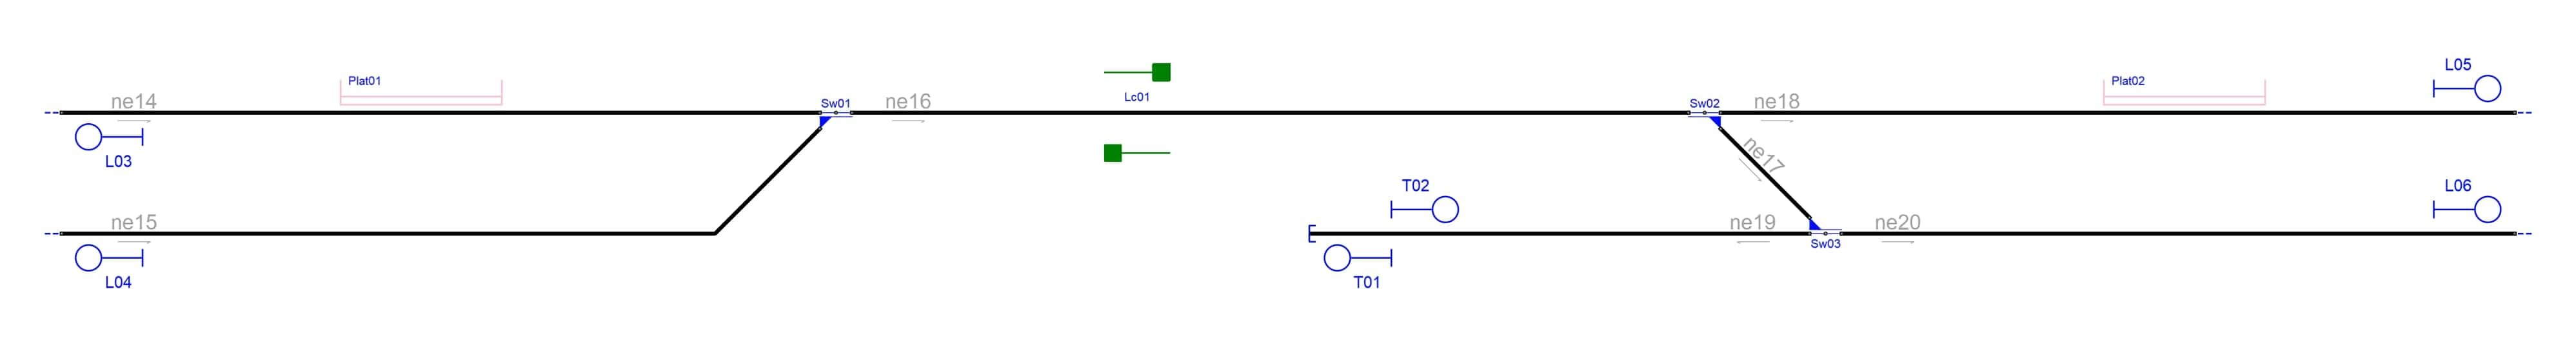
\includegraphics[width=1\textwidth]{resultados-obtenidos/ejemplo2/images/2_step2.png}
		\centering\caption{Señalamiento generado por el RNA para proteger las junturas.}
		\label{fig:EJ2_3}
	\end{figure}
	
	Al generar el señalamiento para proteger la infraestructura, tal como se explicó en la Sección \ref{sec:horizontal}, el Algoritmo \ref{alg:horizontal} simplificará las señales entre dos elementos ferroviarios si no existe espacio suficiente entre ellos. Esto no ocurre con la infraestructura de este ejemplo, ya que las plataformas Plat01 y Plat02, y el cruce de vías Lc01 se encuentran lo suficientemente espaciados entre sí. El señalamiento generado para proteger las plataformas y los cruces de vía se ilustra en rojo en la Figura \ref{fig:EJ2_5}. Las señales generadas para proteger las plataformas son las señales de partida P09, P10, P11 y P12, mientras que las señales que protegen los cruces de vía son las señales X07 y X08.
	
	\begin{figure}[H]
		\centering
		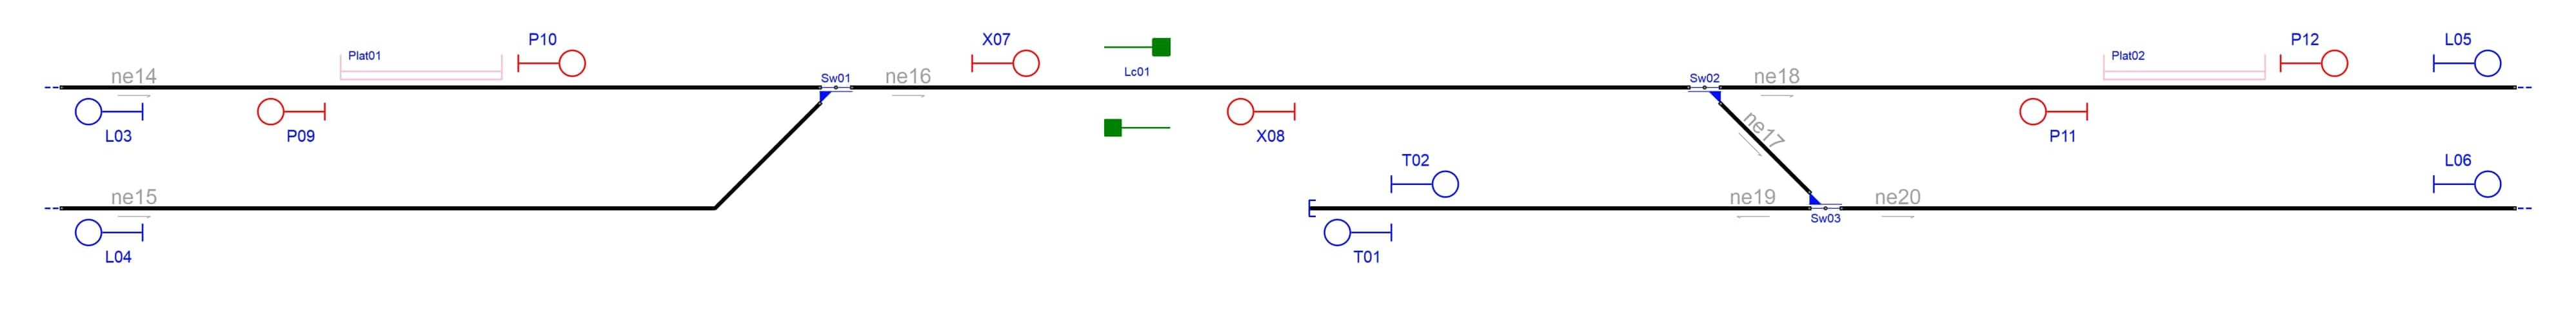
\includegraphics[width=1\textwidth]{resultados-obtenidos/ejemplo2/images/2_step3.png}
		\centering\caption{Señalamiento generado por el RNA para proteger plataformas y cruces de vía.}
		\label{fig:EJ2_5}
	\end{figure}

	El RNA generó las señales C13, B14, S18 y H19 para proteger el cambio de vías Sw01; las señales C17, S15 y H16 para proteger el cambio de vías Sw02; y las señales C20, S21 y H22 para proteger el cambio de vías Sw03. Las señales mencionadas se encuentran resaltadas en rojo en la Figura \ref{fig:EJ2_6}.

	 \begin{figure}[H]
		\centering
		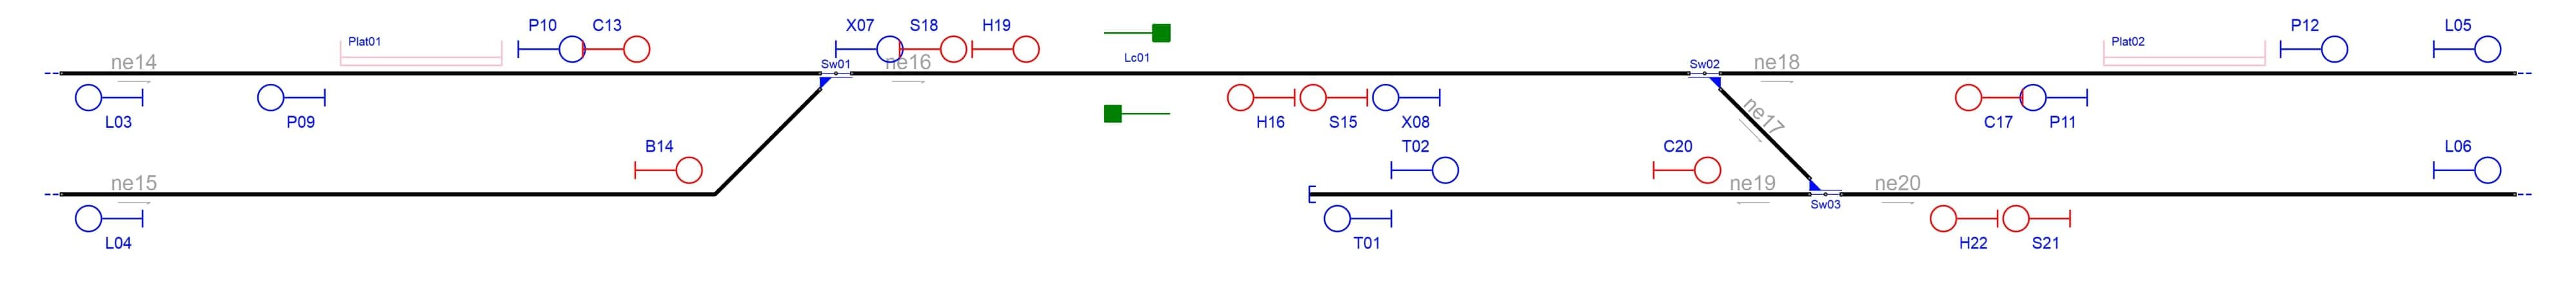
\includegraphics[width=1\textwidth]{resultados-obtenidos/ejemplo2/images/2_step4.png}
		\centering\caption{Señalamiento generado por el RNA para proteger las máquinas de cambios.}
		\label{fig:EJ2_6}
	\end{figure}

	Una vez obtenido todo el señalamiento, el RNA procede a simplificar las señales redundantes, repetidas o cuyas funciones o ubicaciones se superponen entre sí. El proceso de simplificación de señales fue explicado en la Sección \label{sec:simplificacion}. El Algoritmo \ref{alg:vertical} de herencia vertical fue aplicado en las señales B entre los cambios de vías Sw02 y Sw03, desplazando las señales hasta convertirlas en las señales H16 y H22 respectivamente.
	
	Las señales simplificadas al aplicar el Algoritmo \ref{alg:horizontal} de herencia horizontal son: L03, L05, X07, X08, C13, C17 y C20. La señal L03 fue eliminada por su cercanía con la señal P09, con la cual comparte dirección y sentido. Lo mismo ocurre entre la señal L05 y la señal P12; entre las señales C17 y P11; y entre las señales C20 y T02. En todos los casos, se aplicó el Algoritmo \ref{alg:horizontal}, diseñado para agrupar objetos cercanos como un único objeto, generando el señalamiento acorde a los elementos contenidos en cada extremo del nuevo elemento contenedor.
	
	Finalmente, las señales X08 y X09 fueron simplificadas aplicando el Algoritmo \ref{alg:horizontal} de herencia horizontal entre las señales S18 y S15 respectivamente. El resultado final, luego de aplicar el Algoritmo \ref{alg:reduction} de eliminación por prioridad de señales es detallado en el Código \ref{lst:EJ2_3}.

	\begin{lstlisting}[language = {}, caption = Reducción de señalamiento por prioridad de señales, label = {lst:EJ2_3}]
	removing sig20 for sig02
	removing sig03 for sig09
	removing sig05 for sig12
	removing sig07 for sig18
	removing sig08 for sig15
	removing sig13 for sig10
	removing sig17 for sig11
	removing sig16 for sig08
	removing sig19 for sig07
	removing sig22 for sig21
	\end{lstlisting}

	El resultado de la simplificación del señalamiento se ilustra en la Figura \ref{fig:EJ2_7}.

	 \begin{figure}[H]
		\centering
		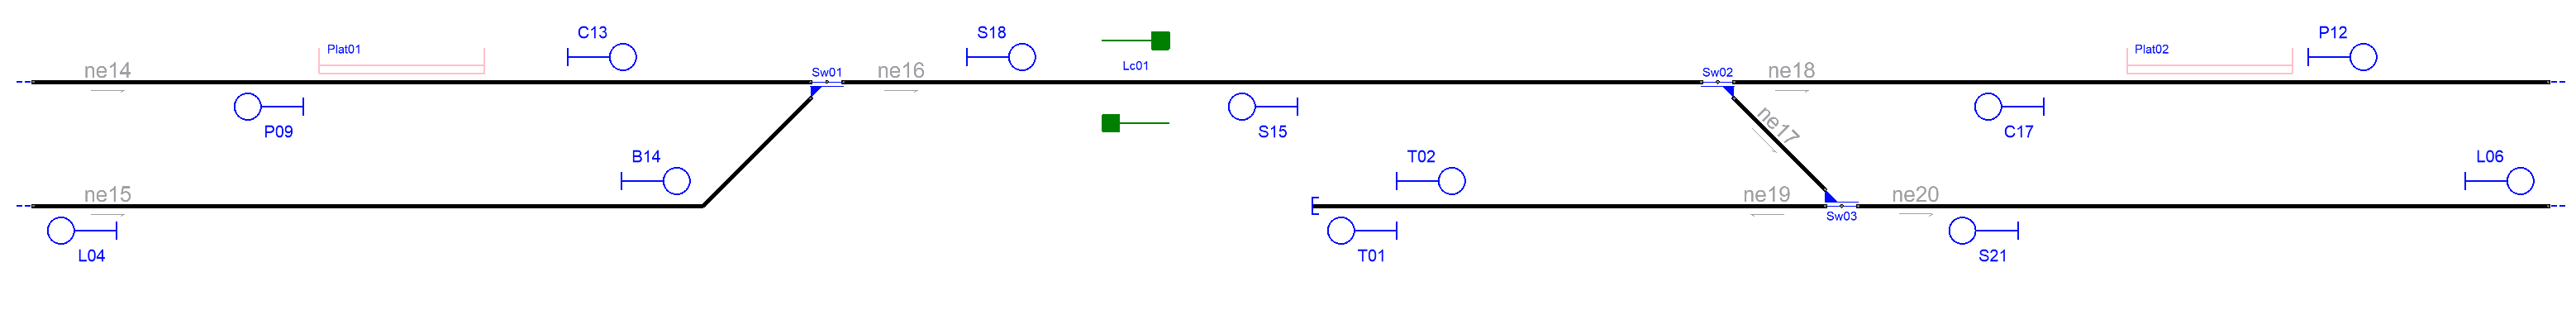
\includegraphics[width=1\textwidth]{resultados-obtenidos/ejemplo2/images/2_RNA.png}
		\centering\caption{Señalamiento generado y simplificado por el RNA.}
		\label{fig:EJ2_7}
	\end{figure}
	
	Al finalizar la generación del señalamiento, el RNA debe detectar todas las posibles rutas admitidas por la red para crear la tabla de enclavamientos. El RNA exporta los resultados del análisis en los siguientes cuatro documentos:
	
	Infrastructure.RNA (Código \ref{lst:EJ2_4}): resumen de cada elemento ferroviario en cada \textit{netElement}.

	\begin{lstlisting}[language = {}, caption = Infrastructure.RNA, label = {lst:EJ2_4}]
	Nodes: 7|Switches: 3|Signals: 0|Detectors: 0|Ends: 5|Barriers: 1
	Node ne14:
	Track = track2
	Neighbours = 2 -> ['ne16', 'ne15']
	Node ne15:
	Track = track3
	Neighbours = 2 -> ['ne14', 'ne16']
	Node ne16:
	Track = track1
	Neighbours = 4 -> ['ne14', 'ne15', 'ne18', 'ne17']
	Level crossing -> lcr120
	Protection -> true | Barriers -> none | Lights -> none Acoustic -> none
	Position -> [-147, -450] | Coordinate: 0.3839
	Switches -> Sw01
	ContinueCourse -> right -> ne14
	BranchCourse -> left -> ne15
	Switches -> Sw02
	ContinueCourse -> left -> ne18
	BranchCourse -> right -> ne17
	Node ne17:
	Track = track5
	Neighbours = 4 -> ['ne16', 'ne18', 'ne20', 'ne19']
	Node ne18:
	Track = track4
	Neighbours = 2 -> ['ne16', 'ne17']
	Node ne19:
	Track = track7
	Type = BufferStop -> ['bus88']
	Neighbours = 2 -> ['ne17', 'ne20']
	Node ne20:
	Track = track6
	Neighbours = 2 -> ['ne17', 'ne19']
	Switches -> Sw03
	ContinueCourse -> left -> ne19
	BranchCourse -> right -> ne17
	\end{lstlisting}

	SafePoints.RNA (Código \ref{lst:EJ2_5}): coordenadas absolutas de cada punto donde puede colocarse una señal, en cada \textit{netElement}.

	\begin{lstlisting}[language = {}, caption = SafePoints.RNA, label = {lst:EJ2_5}]
	ne14:
	Next: [[-1275, -450]]
	Prev: [[-875, -450]]
	ne15:
	Next: [[-810.0, 300]]
	ne16:
	Next: [[-392, -450]]
	Prev: [[8, -450]]
	ne18:
	Next: [[911, -450]]
	Prev: [[1311, -450]]
	ne19:
	Next: [[240.7, 300], [453.3, 300]]
	Prev: [[240.7, 300], [453.3, 300]]
	ne20:
	Next: [[879.8, 300], [1093.5, 300], [1307.2, 300]]
	Prev: [[879.8, 300], [1093.5, 300], [1307.2, 300]]
	\end{lstlisting}

	Signalling.RNA (Código \ref{lst:EJ2_6}): información detallada de todas las señales generadas.

	\begin{lstlisting}[language = {}, caption = Signalling.RNA, label = {lst:EJ2_6}]
	sig01 [T01] <<:
	From: ne19 | To: bus88_left
	Type: Stop | Direction: normal | AtTrack: left 
	Position: [128, -300] | Coordinate: 0.1567
	sig02 [T02] >>:
	From: ne19 | To: ne19_right
	Type: Stop | Direction: reverse | AtTrack: right 
	Position: [128, -300] | Coordinate: 0.1567
	sig04 [L04] <<:
	From: ne15 | To: line113_left
	Type: Circulation | Direction: reverse | AtTrack: right 
	Position: [-1421, -300] | Coordinate: 0.3050
	sig06 [L06] >>:
	From: ne20 | To: line115_right
	Type: Circulation | Direction: normal | AtTrack: left 
	Position: [1421, -300] | Coordinate: 0.8830
	sig09 [P09] <<:
	From: ne14 | To: ne14_left
	Type: Circulation | Direction: reverse | AtTrack: right 
	Position: [-1195, 450] | Coordinate: 0.9960
	sig10 [P10] >>:
	From: ne14 | To: ne14_right
	Type: Circulation | Direction: normal | AtTrack: left 
	Position: [-955, 450] | Coordinate: 1.1063
	sig11 [P11] <<:
	From: ne18 | To: ne18_left
	Type: Circulation | Direction: reverse | AtTrack: right 
	Position: [991, 450] | Coordinate: 1.0125
	sig12 [P12] >>:
	From: ne18 | To: ne18_right
	Type: Circulation | Direction: normal | AtTrack: left 
	Position: [1231, 450] | Coordinate: 1.1437
	sig14 [B14] >>:
	From: ne15 | To: ne15_right
	Type: Manouver | Direction: normal | AtTrack: left 
	Position: [-810.0, -300] | Coordinate: 0.9022
	sig15 [S15] <<:
	From: ne16 | To: ne16_left
	Type: Circulation | Direction: reverse | AtTrack: right 
	Position: [8, 450] | Coordinate: 0.9890
	sig18 [S18] >>:
	From: ne16 | To: ne16_right
	Type: Circulation | Direction: normal | AtTrack: left 
	Position: [-392, 450] | Coordinate: 0.8508
	sig21 [S21] <<:
	From: ne20 | To: ne20_left
	Type: Circulation | Direction: reverse | AtTrack: right 
	Position: [879.8, -300] | Coordinate: 0.2500
	\end{lstlisting}

	Routes.RNA (Código \ref{lst:EJ2_7}): tabla de enclavamientos.
	
	\begin{lstlisting}[language = {}, caption = Routes.RNA, label = {lst:EJ2_7}]
	route_1 [sig02 >> sig06]:
	Path: ['ne19', 'ne20']
	Switches: ['Sw03']
	route_2 [sig10 >> sig18]:
	Path: ['ne14', 'ne16']
	Switches: ['Sw01', 'Sw02']
	Platforms: ['plf116']
	route_3 [sig11 << sig15]:
	Path: ['ne18', 'ne16']
	Switches: ['Sw01', 'Sw02']
	Platforms: ['plf117']
	route_4 [sig14 >> sig18]:
	Path: ['ne15', 'ne16']
	Switches: ['Sw01', 'Sw02']
	route_5 [sig15 << sig09]:
	Path: ['ne16', 'ne14']
	Switches: ['Sw01', 'Sw02']
	Platforms: ['plf116']
	route_6 [sig15 << sig04]:
	Path: ['ne16', 'ne15']
	Switches: ['Sw01', 'Sw02']
	route_7 [sig18 >> sig12]:
	Path: ['ne16', 'ne18']
	Switches: ['Sw01', 'Sw02']
	Platforms: ['plf117']
	route_8 [sig18 >> sig06]:
	Path: ['ne16', 'ne17', 'ne20']
	Switches: ['Sw01', 'Sw02', 'Sw03']
	route_9 [sig21 << sig15]:
	Path: ['ne20', 'ne17', 'ne16']
	Switches: ['Sw01', 'Sw02', 'Sw03']
	route_10 [sig21 << sig01]:
	Path: ['ne20', 'ne19']
	Switches: ['Sw03']
	\end{lstlisting}
	

















